\documentclass[12pt,a4paper]{article}
\usepackage[utf8]{inputenc}
\usepackage[T1]{fontenc}
\usepackage{amsmath}
\usepackage{amsfonts}
\usepackage{amssymb}
\usepackage{graphicx}
\usepackage[indonesian]{babel}
\usepackage[left=2.00cm, right=2.00cm, top=2.00cm, bottom=2.00cm]{geometry}
\usepackage{float} 

\title{Tugas 14 - Pengolahan Sinyal Digital\\
	Disain Filter Digital IIR}

% remove spacing around date:
\usepackage{titling}
\predate{}
\postdate{}
\date{}

\begin{document}
	\maketitle
	\date{}
	\begin{enumerate}
		\item Diketahui frekuensi response dari filter digital yang ditunjukkan oleh Gambar 
		
		\begin{figure}[H]
			\centering
			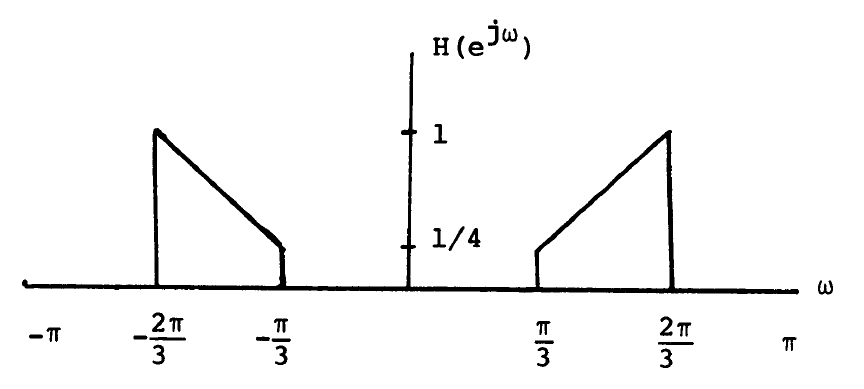
\includegraphics[width=0.7\linewidth]{img/img01}
			\caption{}
			\label{fig:img01}
		\end{figure}
		
		\begin{enumerate}
			\item Tentukan dan gambarkan karakteristik respons frekuensi analog yang, tanpa aliasing, akan dipetakan ke respons frekuensi digital ini ketika dilakukan transformasi impuls invarian.
			\item Gambarkan frekuensi response analog yang akan memetakan response frekuensi digital ini ketika diberikan transformasi bilinear.
		\end{enumerate}
	
	\end{enumerate}
\end{document}